\documentclass[../240906_cryptlab_flute.tex]{subfiles}

\begin{document}

\subsection{Calculating LUT}
\begin{frame}{}
    \begin{exampleblock}{}
        \begin{description}[Output]
            \ii[Input]
            \(\lang\cdot\rang\)-shares of \(\vec{u}^1, \cdots, \vec{u}^M \in (\ZZ_2)^N\),
            \([\cdot]\)-shares of \(\lambda_{\mcal{Q}}\) for each \(\mcal{Q} \subseteq \mcal{I}_k\)
            with \(|\mcal{Q}| > 1\) where \(\mcal{I}_k = \{\,\vec{u}^1_k,\cdots,\vec{u}^M_k\,\}\)
            for \(k \in [N]\),
            and \([\cdot]\)-sharing of \(\lambda_z\).
            \ii[Output]
            \(\lang\cdot\rang\)-shares of
            \(z \coloneqq \vec{u}^1 \odot \cdots \odot \vec{u}^M = \bigoplus_{k=1}^N \bigwedge_{j=1}^M \vec{u}^j_k\).
        \end{description}
        With the prepared \ul{\(N(2^M - M - 1)\) multiplication triples},
        a \(\lang\cdot\rang\)-share of \(\bigodot_{j=1}^N \vec{u}^j\)
        is calculated with the cost of two bits in a single round.
    \end{exampleblock}

    \pause
    \begin{columns}
        \begin{column}{.5\textwidth}
            \begin{equation*}
                y
                = \begin{pmatrix} \ol{x_1} \\ \ol{x_1} \\ x_1 \end{pmatrix}
                   \odot \begin{pmatrix} \ol{x_2} \\ x_2 \\ \ol{x_2} \end{pmatrix}
                   \odot \begin{pmatrix} \ol{x_3} \\ x_3 \\ x_3 \end{pmatrix}
            \end{equation*}
        \end{column}
        \begin{column}{.5\textwidth}
            \centering
            For \(\delta\)-to-\(1\) LUT, \\
            \(N \le 2^{\delta - 1}\) and \(M = \delta\)?? \\
            \pause
            \(2^{\delta-1}(2^\delta-\delta-1)\) triples??
        \end{column}
    \end{columns}

    \pause
    \begin{alertblock}{}
        We now exploit the fact that elements of \(\vec{u}^j\) are closely related.
        \centerline{\fbox{\(\lambda_v\) is unchanged when calculating shares of \(\ol{v}\)!}}
    \end{alertblock}
\end{frame}

\begin{frame}{Some Definitions}
    Fix a \(\delta\)-to-\(\sigma\) LUT \(\Table\).
    \begin{columns}
        \begin{column}{.5\textwidth}
            \begin{figure}[H]
                \centering
                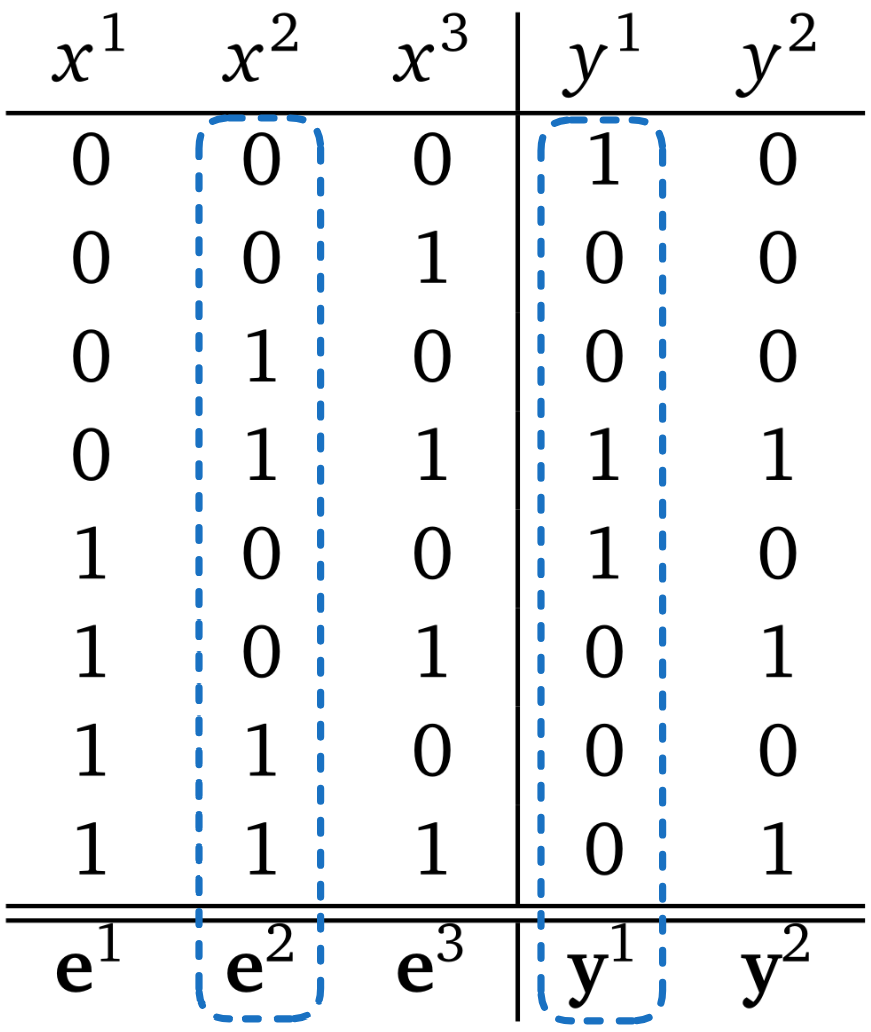
\includegraphics[width=.7\linewidth]{../images/example_table.png}
            \end{figure}
            % \begin{table}[]
            % \begin{tabular}{ccc|cc}
            % \(x^1\) & \(x^2\) & \(x^3\) & \(y^1\) & \(y^2\) \\ \hline
            % \(0\)   & \(0\)   & \(0\)   & \(1\)   & \(0\)   \\
            % \(0\)   & \(0\)   & \(1\)   & \(0\)   & \(0\)   \\
            % \(0\)   & \(1\)   & \(0\)   & \(0\)   & \(0\)   \\
            % \(0\)   & \(1\)   & \(1\)   & \(1\)   & \(1\)   \\
            % \(1\)   & \(0\)   & \(0\)   & \(1\)   & \(0\)   \\
            % \(1\)   & \(0\)   & \(1\)   & \(0\)   & \(1\)   \\
            % \(1\)   & \(1\)   & \(0\)   & \(0\)   & \(0\)   \\
            % \(1\)   & \(1\)   & \(1\)   & \(0\)   & \(1\)   \\ \hline\hline
            % \(\vec{e}^1\) & \(\vec{e}^2\) & \(\vec{e}^3\) & \(\vec{y}^1\) & \(\vec{y}^2\)
            % \end{tabular}
            % \end{table}
        \end{column}
        \begin{column}{.5\textwidth}
            For instance, in this example,
            \[
                \vec{e}^2 = \begin{pmatrix} 0 \\ 0 \\ 1 \\ 1 \\ 0 \\ 0 \\ 1 \\ 1 \end{pmatrix}
                \quad\text{and}\quad
                \vec{y}^1 = \begin{pmatrix} 1 \\ 0 \\ 0 \\ 1 \\ 1 \\ 0 \\ 0 \\ 0 \end{pmatrix}.
            \]
        \end{column}
    \end{columns}
\end{frame}

\subsection{Expressing LUT with Multi-Fan-In Inner Product}
\begin{frame}{Expressing LUT with Multi-Fan-In Inner Product}
    Now, in the previous example, note that:
    \begin{columns}
        \begin{column}{.4\textwidth}
            \begin{table}[H]
                \centering
                \begin{tabular}{ccc|c}
                \(x^1\) & \(x^2\) & \(x^3\) & \(y^1\) \\ \hline
                \(0\)   & \(0\)   & \(0\)   & \(1\)   \\
                \(0\)   & \(0\)   & \(1\)   & \(0\)   \\
                \(0\)   & \(1\)   & \(0\)   & \(0\)   \\
                \(0\)   & \(1\)   & \(1\)   & \(1\)   \\
                \(1\)   & \(0\)   & \(0\)   & \(0\)   \\
                \(1\)   & \(0\)   & \(1\)   & \(1\)   \\
                \(1\)   & \(1\)   & \(0\)   & \(0\)   \\
                \(1\)   & \(1\)   & \(1\)   & \(0\)  
                \end{tabular}
            \end{table}
        \end{column}
        \begin{column}{.5\textwidth}
            \small
            \begin{align*}
                \vec{z}^1
                &= \begin{pmatrix} \ol{x^1} \\ \ol{x^1} \\ x^1 \end{pmatrix}
                   \odot \begin{pmatrix} \ol{x^2} \\ x^2 \\ \ol{x^2} \end{pmatrix}
                   \odot \begin{pmatrix} \ol{x^3} \\ x^3 \\ x^3 \end{pmatrix} \\
                &= \begin{pmatrix} \ol{x^1} \\ \ol{x^1} \\ \ol{x^1} \\ \ol{x^1} \\ \vdots \end{pmatrix}
                   \odot \begin{pmatrix} \ol{x^2} \\ \ol{x^2} \\ x^2 \\ x^2 \\ \vdots \end{pmatrix}
                   \odot \begin{pmatrix} \ol{x^3} \\ x^3 \\ \ol{x^3} \\ x^3 \\ \vdots \end{pmatrix}
                   \odot \begin{pmatrix} 1 \\ 0 \\ 0 \\ 1 \\ \vdots \end{pmatrix} \\
                &= (\ol{x^1} \oplus \vec{e}^1) \odot \cdots \odot (\ol{x^3} \oplus \vec{e}^3) \odot \vec{y}^1
            \end{align*}
            \footnoterule
            \footnotesize
            \(\ol{x^j} \oplus \vec{e}^j\) is an element-wise addition.
        \end{column}
    \end{columns}
\end{frame}

\begin{frame}{Expressing LUT with Multi-Fan-In Inner Product}
    \begin{block}{}
    Fixing a \(\delta\)-to-\(\sigma\) LUT \(\Table\),
    and given \(\lang\cdot\rang\)-shares of \(x^1, \cdots, x^\delta\),
    let
    \[
        \vec{u}^j \coloneqq \ol{x^j} \oplus \vec{e}^j \in (\ZZ_2)^{2^\delta}
    \]
    for \(j \in [\delta]\) so that
    \[
        \lang \vec{u}^j_k \rang_i = \left(\ol{\msf{m}_{x^j}} \oplus \vec{e}^j_k, [\lambda_{x^j}]_i\right)
    \]
    gives a \(\lang\cdot\rang\)-sharing of \(\vec{u}^j_k\) for \(j \in [\delta]\), \(k \in [2^\delta]\).
    \end{block}
    \pause
    \begin{exampleblock}{}
        With this, we have
        \[
            \lambda_{\vec{u}^{j_1}_{k_1}\cdots\vec{u}^{j_n}_{k_n}}
            = \lambda_{x^{j_1} \cdots x^{j_n}}\text{!}
        \]
    \end{exampleblock}
\end{frame}

\begin{frame}{Expressing LUT with Multi-Fan-In Inner Product}
    As previously shown, the \(w\)-th output \(\vec{z}^w\) can be calculated by
    \begin{align*}
        \vec{z}^w
        &= (\ol{x^1} \oplus \vec{e}^1) \odot \cdots \odot (\ol{x^\delta} \oplus \vec{e}^\delta) \odot \vec{y}^w \\
        &= \vec{u}^1 \odot \cdots \odot \vec{u}^\delta \odot \vec{y}^w \\
        &= \bigoplus_{k=1}^{2^\delta} \left[ \left(\bigwedge_{j=1}^\delta \vec{u}^j_k\right) \wedge \vec{y}^w_k \right] \\
        &= \bigoplus_{k=1}^{2^\delta} \left[
            \left(\bigwedge_{j=1}^\delta \left( \msf{m}_{\vec{u}^j_k} \oplus \lambda_{\vec{u}^j_k} \right) \right)
            \wedge \vec{y}^w_k \right] \\
        &= \bigoplus_{k=1}^{2^\delta} \left[\vec{y}^w_k \cdot \bigoplus_{\mcal{Q}_k \subseteq \mcal{I}_k}
            \big(\msf{m}_{\mcal{Q}_k} \cdot \lambda_{\mcal{I}_k \setminus \mcal{Q}_k} \big)\right]
    \end{align*}
    where \(\mcal{I}_k \coloneqq \{\,\vec{u}^1_k, \cdots, \vec{u}^\delta_k\,\}\)
    for each \(k \in [2^\delta]\).
\end{frame}

\subsection{Calculating LUT}
\begin{frame}{Calculating LUT}
    \begin{block}{Calculating \(\delta\)-to-\(\sigma\) LUT}
        \begin{description}[Output]
            \ii[Input]
            A \(\delta\)-to-\(\sigma\) LUT \(\Table\),
            \(\lang\cdot\rang\)-shares of \(x^1, \cdots, x^\delta \in \ZZ_2\),
            \([\cdot]\)-shares of \(\lambda_{\mcal{Q}}\) for each \(\mcal{Q} \subseteq \mcal{I}\)
            with \(|\mcal{Q}| > 1\) where \(\mcal{I} = \{x^1,\cdots,x^\delta\}\), and
            \([\cdot]\)-shares of \(\lambda_z\).
            \ii[Output]
            \(\lang\cdot\rang\)-shares of \(z \coloneqq \Table(x^1, \cdots, x^\delta)\).
        \end{description}
        \pause
        \begin{enumerate}
            \ii
            \(P_i\) computes its share of \(\vec{u}^j_k = \ol{x^j} \oplus \vec{e}^j_k\)
            for \(j \in [\delta]\) and \(k \in [2^\delta]\).
            \pause
            \ii
            \(P_i\) computes, for each \(w \in [\sigma]\),
            \centerline{%
                \(\displaystyle
                [\vec{z}_w]_i = i \cdot \bigoplus_{k=1}^{2^\delta} (\vec{y}^w_k \cdot \msf{m}_{\mcal{I}_k})
                \oplus \bigoplus_{k=1}^{2^\delta} \left[
                    \vec{y}^w_k \cdot \bigoplus_{\mcal{Q}_k \subsetneq \mcal{I}_k} \big(
                    \msf{m}_{\mcal{Q}_k} \cdot [\lambda_{\mcal{I}_k \setminus \mcal{Q}_k}]_i \big)
                \right].
                \)
            }
            \pause
            \ii
            \(P_i\) computes \([\msf{m}_{\vec{z}_w}]_i = [\vec{z}_w]_i \oplus [\lambda_{\vec{z}_w}]_i\)
            for \(w \in [\sigma]\) and sends them to \(P_{1-i}\).
            \ii
            Then, \(P_0\) and \(P_1\) have \(\lang\cdot\rang\)-shares of \(\vec{z} = \Table(x^1, \cdots, x^\delta)\).
        \end{enumerate}
    \end{block}
\end{frame}

\begin{frame}{Calculating LUT}
    \begin{block}{Calculating \(\delta\)-to-\(\sigma\) LUT}
        \begin{description}[Output]
            \ii[Input]
            A \(\delta\)-to-\(\sigma\) LUT \(\Table\),
            \(\lang\cdot\rang\)-shares of \(x^1, \cdots, x^\delta \in \ZZ_2\),
            \([\cdot]\)-shares of \(\lambda_{\mcal{Q}}\) for each \(\mcal{Q} \subseteq \mcal{I}\)
            with \(|\mcal{Q}| > 1\) where \(\mcal{I} = \{x^1,\cdots,x^\delta\}\), and
            \([\cdot]\)-shares of \(\lambda_z\).
            \ii[Output]
            \(\lang\cdot\rang\)-shares of \(z \coloneqq \Table(x^1, \cdots, x^\delta)\).
        \end{description}
        With the prepared \(2^\delta - \delta - 1\) multiplication triples,
        a \(\lang\cdot\rang\)-share of \(\Table(x^1, \cdots, x^\delta)\)
        is calculated with the cost of \ul{\(2\sigma\) bits in a single round}.
    \end{block}
\end{frame}

\subsection{Pros and Cons}
\begin{frame}{Pros and Cons}
    \begin{block}{Pros}
        \begin{itemize}
            \ii Any complex circuit can be represented by an \emph{interconnection of small LUTs}.
            \ii Evaluation does not depend on the internal logic.
            \ii Setup does not depend on the number of outputs.
        \end{itemize}
    \end{block}
    \pause
    \begin{block}{Cons}
        \begin{itemize}
            \ii Exponential setup time/communicaion.
            \ii Exponential internal calculation.
        \end{itemize}
    \end{block}
\end{frame}

\end{document}
